\documentclass[11pt,letterpaper]{article}

% ── Fonts ─────────────────────────────────────────────────────────
\usepackage[T1]{fontenc}
\usepackage{newtxtext}
\usepackage{amssymb}
\usepackage{newtxmath}
\usepackage[scaled=0.85]{inconsolata}

% ── Layout ────────────────────────────────────────────────────────
\usepackage[margin=1in]{geometry}
\usepackage{setspace}
\setstretch{1.08}
\usepackage{parskip}
\setlength{\parskip}{0.5\baselineskip plus 2pt minus 1pt}

% ── Section headings ──────────────────────────────────────────────
\usepackage{titlesec}
\titleformat{\section}{\large\bfseries}{\thesection}{1em}{}
\titleformat{\subsection}{\normalsize\bfseries}{\thesubsection}{0.8em}{}
\titleformat{\subsubsection}{\normalsize\itshape}{\thesubsubsection}{0.8em}{}
\titlespacing*{\section}{0pt}{1.8ex plus 0.5ex}{0.8ex plus 0.2ex}
\titlespacing*{\subsection}{0pt}{1.4ex plus 0.3ex}{0.4ex plus 0.1ex}

% ── Math ──────────────────────────────────────────────────────────
\usepackage{amsmath}
\usepackage{mathtools}
\let\openbox\relax
\usepackage{amsthm}

% ── Tables ────────────────────────────────────────────────────────
\usepackage{booktabs}
\usepackage{array}
\usepackage{tabularx}
\renewcommand{\arraystretch}{1.15}
\usepackage{caption}
\captionsetup{font=small, labelfont=bf, labelsep=period, skip=6pt}
\captionsetup[table]{position=above}

% ── Floats ───────────────────────────────────────────────────────
\usepackage{float}
\usepackage{graphicx}
\setlength{\floatsep}{6pt plus 2pt minus 2pt}
\setlength{\textfloatsep}{8pt plus 2pt minus 2pt}
\setlength{\intextsep}{6pt plus 2pt minus 2pt}

% ── Lists ─────────────────────────────────────────────────────────
\usepackage{enumitem}
\setlist{nosep, leftmargin=1.5em}

% ── Colors & Links ────────────────────────────────────────────────
\usepackage{xcolor}
\definecolor{linkblue}{HTML}{0B5394}
\definecolor{citegreen}{HTML}{1B7340}
\definecolor{urlgray}{HTML}{444444}

% ── TikZ (diagrams) ──────────────────────────────────────────────
\usepackage{tikz}
\usetikzlibrary{arrows.meta, positioning, shapes.geometric, calc, decorations.pathreplacing, fit}

\usepackage[
  colorlinks=true,
  linkcolor=linkblue,
  citecolor=citegreen,
  urlcolor=urlgray,
  bookmarksnumbered=true,
  pdfstartview=FitH,
]{hyperref}
\usepackage[noabbrev,capitalise]{cleveref}

% ── Microtypography ──────────────────────────────────────────────
\usepackage{microtype}

% ── Theorem environments ─────────────────────────────────────────
\newtheorem{proposition}{Proposition}

% ══════════════════════════════════════════════════════════════════
\title{\textbf{When More Data Hurts:\\[2pt]
  A Directional Goodhart Condition for\\[2pt]
  Multi-Stakeholder Preference Learning}}
\author{Kartik G Bhat\thanks{Independent Researcher. Contact: \texttt{gkartik@gmail.com}}}
\date{}

\begin{document}
\maketitle

% ══════════════════════════════════════════════════════════════════
\begin{abstract}\noindent
Multi-stakeholder recommendation systems optimize proxy objectives
that may harm unobserved stakeholders. We identify a precise
condition governing when this occurs: in Bradley-Terry preference
learning with $K$ stakeholders, additional training data degrades a
hidden stakeholder's \emph{expected} utility if and only if the cosine
similarity between the BT-trained weight vectors of the optimization
target and the hidden stakeholder is negative. We validate this
\emph{directional Goodhart condition} on 32 strong-cosine data points
across 4 datasets (MovieLens-100K, MovieLens-1M, MIND, Amazon Kindle),
13 stakeholders, and 3 feature families ($D \in \{19, 32, 35\}$), with
100\% accuracy for $|\cos| > 0.2$ (32/32) under softmax-weighted
evaluation and 91\% (29/32) under hard top-$K$ selection. The
condition correctly predicts that X's 18-action engagement space
exhibits no Goodhart effect (all stakeholder pairs have positive
cosine), correcting a prior Hausdorff-based analysis that falsely
indicated otherwise.

Two precisions emerge from the cross-dataset analysis. First, the
relevant cosine is between BT-\emph{trained} weight vectors, not raw
stakeholder weights; on high-dimensional sparse features, BT training
remaps the cosine geometry (up to 3 of~10 pairs flip sign on MIND).
Second, the condition governs expected utility under the learned score
distribution; under hard top-$K$ selection, it can reverse for
stakeholders with high utility variance near the selection boundary
(5 of~20 MIND pairs, 0 of~8 Amazon, 0 of~6 MovieLens). The reversal
vanishes at softmax temperature $T \geq 1$.
Applied to X's open-sourced recommendation algorithm, the Goodhart
risk reduces to one observable: whether the platform treats negative
signals (blocks, reports) as positive engagement. We provide an audit
toolkit, a data budget analysis (median 33 preference pairs to recover
50\% of hidden stakeholder harm across 13 stakeholder configurations),
and practical guidance for platform transparency under the EU Digital
Services Act.
\end{abstract}

%═══════════════════════════════════════════════════════════════════
\section{Introduction}
\label{sec:intro}
%═══════════════════════════════════════════════════════════════════

% TODO: Write after §4 and §6
\textit{[Introduction placeholder.]}

%═══════════════════════════════════════════════════════════════════
\section{Background and Related Work}
\label{sec:background}
%═══════════════════════════════════════════════════════════════════

% TODO: Adapt from old preprint §2, add Gao/Kwa
\textit{[Background placeholder.]}

%═══════════════════════════════════════════════════════════════════
\section{Setup}
\label{sec:setup}
%═══════════════════════════════════════════════════════════════════

\subsection{Stakeholder Utility Model}

We consider a recommendation setting with $K$ stakeholders. Each
content item~$c$ is represented by a $D$-dimensional feature
vector~$\mathbf{p}(c)$, and each stakeholder~$k$ assigns utility
\begin{equation}
  U_k(c) = \mathbf{w}_k^\top \mathbf{p}(c),
  \label{eq:utility}
\end{equation}
where $\mathbf{w}_k \in \mathbb{R}^D$ is the stakeholder's weight
vector over features. Different stakeholders express different
preferences through different weights. The angle between two weight
vectors determines their alignment:
$\cos(\mathbf{w}_i, \mathbf{w}_j) > 0$ means roughly aligned;
$\cos < 0$ means opposed.

\subsection{Preference Learning}
\label{sec:bt}

A Bradley-Terry (BT) reward model~\cite{bradley1952rank} learns a
weight vector $\hat{\mathbf{w}} \in \mathbb{R}^D$ from pairwise
preference data by minimizing
\begin{equation}
  \mathcal{L}_{\text{BT}} = -\log \sigma\!\bigl(
    \hat{\mathbf{w}}^\top \mathbf{p}_{\text{pref}}
    - \hat{\mathbf{w}}^\top \mathbf{p}_{\text{rej}}
  \bigr),
  \label{eq:btloss}
\end{equation}
where $\sigma$ is the logistic function and
$(\mathbf{p}_{\text{pref}}, \mathbf{p}_{\text{rej}})$ is a
preference pair. Each pair is constructed by sampling two content
items, scoring them with the labeling stakeholder's utility (plus
Gaussian noise, $\sigma_{\text{noise}} = 0.05$), and assigning the
higher-scoring item as preferred. Training uses Adam with learning
rate 0.01, batch size 64, and 50 epochs. All preference data is
split 80/20 into training and held-out evaluation sets.

To simulate misspecification---a scenario where the optimization
target differs from any stakeholder's true utility---we perturb
the target weight vector with multiplicative Gaussian noise:
$\tilde{\mathbf{w}} = \mathbf{w}_t \odot (1 + \boldsymbol{\epsilon})$,
$\boldsymbol{\epsilon} \sim \mathcal{N}(0, \sigma_p^2 \mathbf{I})$
with $\sigma_p = 0.3$. The BT model trains on preferences labeled by
the perturbed~$\tilde{\mathbf{w}}$, so the learned model approaches
but does not exactly recover the target direction.

\subsection{Datasets and Stakeholders}

We use five datasets spanning four feature spaces (\cref{tab:datasets}).

\paragraph{Synthetic benchmark.}

The first dataset uses X's Phoenix recommendation
system~\cite{xalgorithm2023}, which defines 18 user actions on
content (\cref{tab:actions}). Each content item produces an action
probability vector $\mathbf{p} \in [0,1]^{18}$. We generate 500
content items across 6 topics (technology, sports, politics-left,
politics-right, entertainment, science) and 600 users in 5
archetypes, with action probabilities drawn from calibrated
distributions.

Three stakeholders are defined via the structural family
\begin{equation}
  U_k = \sum_{a \in \text{pos}} w_a \cdot p_a
      - \alpha_k \sum_{a \in \text{neg}} |w_a| \cdot p_a,
  \label{eq:synth_utility}
\end{equation}
where $\alpha_k$ is the \emph{negativity aversion} parameter:
\textbf{user}~($\alpha = 1.0$), equal weight on positive engagement
and discomfort avoidance; \textbf{platform}~($\alpha = 0.3$),
tolerant of negative signals; \textbf{society}~($\alpha = 4.0$),
heavily penalizes block/report/mute as proxies for
harm~\cite{bail2018exposure}. The full 18-parameter weight vectors
are listed in \cref{tab:actions}; the stakeholders differ primarily
through~$\alpha$, a special case of additive
MAUT~\cite{keeney1976decisions}.

\begin{table}[t]
  \caption{The 18 Phoenix actions with positive/negative/neutral
    classification and stakeholder weights. User utility sums
    positive and negative groups (\cref{eq:synth_utility}); neutral
    actions contribute zero. Platform weights all actions positively
    --- the key asymmetry driving stakeholder divergence.}
  \label{tab:actions}
  \centering\small
  \begin{tabular}{llrr}
    \toprule
    \textbf{Action} & \textbf{Class} & \textbf{User wt.} & \textbf{Plat.\ wt.} \\
    \midrule
    follow\_author          & Positive  & 1.2   & 1.0 \\
    favorite                & Positive  & 1.0   & 1.0 \\
    share                   & Positive  & 0.9   & 1.3 \\
    repost                  & Positive  & 0.8   & 1.5 \\
    quote                   & Positive  & 0.6   & 1.3 \\
    reply                   & Positive  & 0.5   & 1.2 \\
    \midrule
    report                  & Negative  & $-$2.5 & 0.2 \\
    block\_author           & Negative  & $-$2.0 & 0.1 \\
    mute\_author            & Negative  & $-$1.5 & 0.1 \\
    not\_interested         & Negative  & $-$1.0 & 0.1 \\
    \midrule
    share\_via\_dm          & Neutral   & ---   & 1.4 \\
    share\_via\_copy\_link  & Neutral   & ---   & 1.2 \\
    profile\_click          & Neutral   & ---   & 0.6 \\
    click                   & Neutral   & ---   & 0.5 \\
    vqv                     & Neutral   & ---   & 0.4 \\
    quoted\_click           & Neutral   & ---   & 0.4 \\
    photo\_expand           & Neutral   & ---   & 0.3 \\
    dwell                   & Neutral   & ---   & 0.2 \\
    \bottomrule
  \end{tabular}
\end{table}

\paragraph{MovieLens-100K and MovieLens-1M.}

For real-data validation, we use MovieLens-100K (100K ratings, 943
users, 1{,}682 movies) and MovieLens-1M (1M ratings, 6{,}040 users,
3{,}952 movies)~\cite{harper2015movielens}. Each movie has a binary
genre vector over $D = 19$ genres (Action, Adventure, Animation,
\ldots, Western). Content features are
$\mathbf{p}(c) = \mathbf{g}(c) \cdot \bar{r}(c)/5$, where
$\mathbf{g}(c) \in \{0,1\}^{19}$ is the genre vector and
$\bar{r}(c)$ is the movie's mean rating. Movies with fewer than 5
ratings are excluded, yielding content pools of 1{,}305 (ML-100K)
and 3{,}347 movies (ML-1M).

Three stakeholders are derived from rating data:
\begin{itemize}
  \item \textbf{User}: Genre preference from aggregate rating
    history. $w_g \propto \bar{r}_g - 3$, where $\bar{r}_g$ is the
    mean rating for genre~$g$. Genres rated above average get
    positive weight.
  \item \textbf{Platform}: Popularity-weighted quality.
    $w_g \propto \bar{r}_g \cdot \log_2 n_g$, where $n_g$ is the
    number of ratings in genre~$g$.
  \item \textbf{Diversity}: Anti-concentration.
    $w_g \propto -(f_g - 1/G)$, where $f_g$ is the fraction of
    ratings in genre~$g$ and $G$ is the number of active genres.
    Penalizes dominant genres, rewards rare ones.
\end{itemize}
All weight vectors are normalized to unit maximum absolute value.
The key geometric fact is that user and platform are
strongly aligned ($\cos \approx +0.95$), while both oppose diversity
($\cos \approx -0.3$ to $-0.2$). Five additional stakeholders with
real-world analogs (creator, advertiser, niche enthusiast,
mainstream, content moderator) are introduced in \cref{sec:direction}
to expand validation coverage (MovieLens only; Method~B).

\paragraph{MIND-small.}

For cross-domain validation on news recommendation, we use the
MIND-small dataset~\cite{wu2020mind}: 12{,}261 news articles with
click/impression data. Each article has a $D = 35$ feature vector:
17 top-level news categories (one-hot), 14 top subcategories
(one-hot), and 4 article quality signals (title length, abstract
length, entity count, word count; normalized). Five domain-native
stakeholders are defined:
\textbf{reader} (click-derived category preferences),
\textbf{publisher} (volume and reach),
\textbf{advertiser} (eyeball concentration on popular categories),
\textbf{journalist} (editorial quality signals, investigative
category preference), and
\textbf{civic\_diversity} (anti-concentration across categories,
analogous to MovieLens diversity).
Stakeholder weight construction details are in \cref{app:stakeholders}.

\paragraph{Amazon Kindle Store.}

For e-commerce validation, we use the Amazon Kindle Store
5-core dataset~\cite{ni2019justifying}: 17{,}425 books with
$D = 32$ features (20 genre categories, 4 price-tier indicators,
3 review-volume bins, 3 sentiment-polarity features, 2 text-length
bins). Five stakeholders:
\textbf{reader} (genre preferences from review history),
\textbf{publisher} (catalog breadth and volume),
\textbf{indie\_author} (long-tail genre preference, anti-bestseller),
\textbf{premium\_seller} (price and review-quality signals), and
\textbf{diversity} (anti-concentration, analogous to MovieLens).
Notably, premium\_seller's features occupy slots disjoint from all
other stakeholders, producing 3 pairs with raw cosine exactly~$0.000$
--- a unique probe of the direction condition at the boundary.

\begin{table}[t]
  \caption{Dataset summary. $K$: number of stakeholders.
    $D$: feature dimensionality. Pool: content items after filtering.
    Feature type describes the dominant structure of $\mathbf{p}(c)$.}
  \label{tab:datasets}
  \centering\small
  \begin{tabular}{llrrrl}
    \toprule
    \textbf{Dataset} & \textbf{Domain} & $\boldsymbol{K}$ &
      $\boldsymbol{D}$ & \textbf{Pool} & \textbf{Feature type} \\
    \midrule
    Synthetic     & Social media & 3 & 18 & 500   & Action probs \\
    ML-100K       & Movies       & 3 & 19 & 1{,}305 & Genre $\times$ rating \\
    ML-1M         & Movies       & 3 & 19 & 3{,}347 & Genre $\times$ rating \\
    MIND-small    & News         & 5 & 35 & 12{,}261 & Category one-hot \\
    Amazon Kindle & E-commerce   & 5 & 32 & 17{,}425 & Genre + metadata \\
    \bottomrule
  \end{tabular}
\end{table}

\subsection{Evaluation}
\label{sec:eval}

We evaluate using \emph{per-stakeholder utility on selected
content}, not frontier distance metrics (see \cref{sec:hausdorff}
for why this matters). Given learned weights~$\hat{\mathbf{w}}$, we
sweep a diversity parameter
$\delta \in \{0.0, 0.05, \ldots, 1.0\}$ that controls the tradeoff
between score-based and diversity-based content selection. At each
operating point, a greedy algorithm selects the top-$K = 10$ content
items, and all stakeholder utilities are evaluated on the selected
set. The 21-point sweep traces a Pareto frontier in stakeholder
utility space.

For Goodhart experiments (\cref{sec:direction}), we compare
stakeholder utilities at $N = 25$ and $N = 2{,}000$ training pairs
across 5 random seeds, measuring the percentage change from the
$N = 25$ baseline. The target stakeholder improves by construction;
whether hidden stakeholders improve or degrade is the quantity of
interest. For leave-one-stakeholder-out (LOSO) experiments, we
exclude one stakeholder during training and measure its
\emph{regret}: the utility gap between the full-information Pareto
frontier and the LOSO frontier, averaged across operating points and
20 seeds.

%═══════════════════════════════════════════════════════════════════
\section{The Directional Goodhart Condition}
\label{sec:direction}
%═══════════════════════════════════════════════════════════════════

We train Bradley-Terry reward models on preference pairs labeled by a
misspecified stakeholder utility (the \emph{target}), then measure the
effect on a different stakeholder whose utility was not used in training
(the \emph{hidden} stakeholder). As the number of training pairs~$N$
increases, the BT model converges more precisely toward the target
utility direction. The question is: does this convergence help or hurt
the hidden stakeholder?

\subsection{Statement}

\begin{proposition}[Directional Goodhart Condition]
\label{prop:direction}
In a linear BT preference learning setting with $K$ stakeholders and a
finite content pool~$\mathcal{C}$, let $\hat{\mathbf{w}}_t(N)$ be the
weight vector learned from $N$ preference pairs labeled by target
stakeholder~$t$, and let $\hat{\mathbf{w}}_h$ be the corresponding
BT-learned direction for hidden stakeholder~$h$ (the fixed point of BT
training on~$h$'s labels). Define the expected hidden utility under the
score distribution induced by $\hat{\mathbf{w}}_t(N)$ as
\begin{equation}
  \bar{U}_h(N) \;=\; \sum_{c \in \mathcal{C}}
    \pi_{\hat{\mathbf{w}}_t(N)}(c) \;\cdot\; U_h(c),
  \label{eq:expected_util}
\end{equation}
where $\pi_{\mathbf{w}}(c) \propto
\exp\!\bigl(\mathbf{w}^\top \mathbf{p}(c) / T\bigr)$ is the
softmax selection distribution at temperature~$T$. Then for
sufficiently large~$T$ (empirically, $T \geq 1$):
\begin{itemize}
  \item If\, $\cos(\hat{\mathbf{w}}_t, \hat{\mathbf{w}}_h) < 0$:\;
    $\bar{U}_h(N)$ is eventually decreasing in~$N$.
  \item If\, $\cos(\hat{\mathbf{w}}_t, \hat{\mathbf{w}}_h) > 0$:\;
    $\bar{U}_h(N)$ is eventually increasing in~$N$.
\end{itemize}
\end{proposition}

Two clarifications relative to a na\"{\i}ve formulation. First, the
cosine is computed between \emph{BT-trained} weight vectors, not the
raw stakeholder utility weights. On low-dimensional dense feature
spaces (MovieLens, $D{=}19$), raw and trained cosines agree to within
$\pm 0.05$. On high-dimensional sparse features (MIND, $D{=}35$;
Amazon Kindle, $D{=}32$), BT training can substantially remap the
cosine geometry---up to 3 of~10 pairs flip sign on MIND---and trained
cosines are necessary for reliable prediction. Second, the hidden
utility is evaluated under the \emph{score distribution}
$\pi_{\mathbf{w}}$, not on a hard top-$K$ selection set. Under hard
top-$K$, the condition can reverse for hidden stakeholders with high
utility variance near the selection boundary
(\cref{sec:selection_mechanism}).

In words: more training data degrades a hidden stakeholder's expected
utility if and only if the optimization target is anti-correlated with
that stakeholder in the BT-trained weight space. The condition holds
perfectly for $|\cos| > 0.2$ and has a transition zone near
$\cos \approx 0$ where prediction is unreliable.

\subsection{Empirical Validation}

We validate the direction condition on 32 strong-cosine
($|\cos| > 0.2$) data points across four datasets spanning three
distinct feature families, using BT-trained cosines.

\begin{itemize}
  \item \textbf{MovieLens-100K and MovieLens-1M} ($D{=}19$,
    3 stakeholders each): 6 Method~A pairs per dataset, all with
    $|\text{trained~cos}| > 0.2$. 10 of~10 match (100\%) under both
    top-$K$ and softmax evaluation. Raw and trained cosines agree
    closely on this low-dimensional dense feature space.

  \item \textbf{MIND-small} ($D{=}35$, 5 stakeholders): 20 Method~A
    pairs, of which 14 have $|\text{trained~cos}| > 0.2$. Under
    softmax ($T{=}1.0$): 14/14 match (100\%). Under hard top-10:
    11/14 match (79\%)---the 3 violations all involve one stakeholder
    (journalist) and are explained by the selection mechanism
    (\cref{sec:selection_mechanism}). With raw cosines, only 6 of~10
    strong pairs match (60\%)---the gap is driven by 3 sign flips
    between raw and trained cosines.

  \item \textbf{Amazon Kindle} ($D{=}32$, 5 stakeholders): 20 Method~A
    pairs, of which 8 have $|\text{trained~cos}| > 0.2$. All 8 match
    (100\%) under both mechanisms. Amazon additionally provides
    3 pairs with raw cosine exactly~$0.000$ (orthogonal by
    construction); these stay near zero under BT training
    (max $|\text{trained cos}| = 0.048$), confirming the condition's
    behavior at the boundary.
\end{itemize}

Pooled under softmax evaluation: 32 of 32 strong-cosine pairs match
the predicted direction (100\%). Under hard top-$K$: 29 of 32 (91\%),
with the 3 violations confined to one stakeholder on one dataset. In
the transition zone ($|\cos| < 0.2$), prediction is less reliable,
with violations concentrated near $\cos \approx 0$.

In each experiment, the target stakeholder's weights are perturbed
with multiplicative Gaussian noise ($\sigma = 0.3$). BT models are
trained at $N = 25$ and $N = 2{,}000$ preference pairs. The utility
change from $N = 25$ to $N = 2{,}000$ determines whether the hidden
stakeholder improved or degraded.

On MovieLens, an additional 30 data points from 5 named stakeholders
with real-world analogs (creator, advertiser, niche enthusiast,
mainstream, content moderator) are available via Method~B; these are
dataset-specific and not included in the cross-dataset pooled count.

\begin{figure}[t]
  \centering
  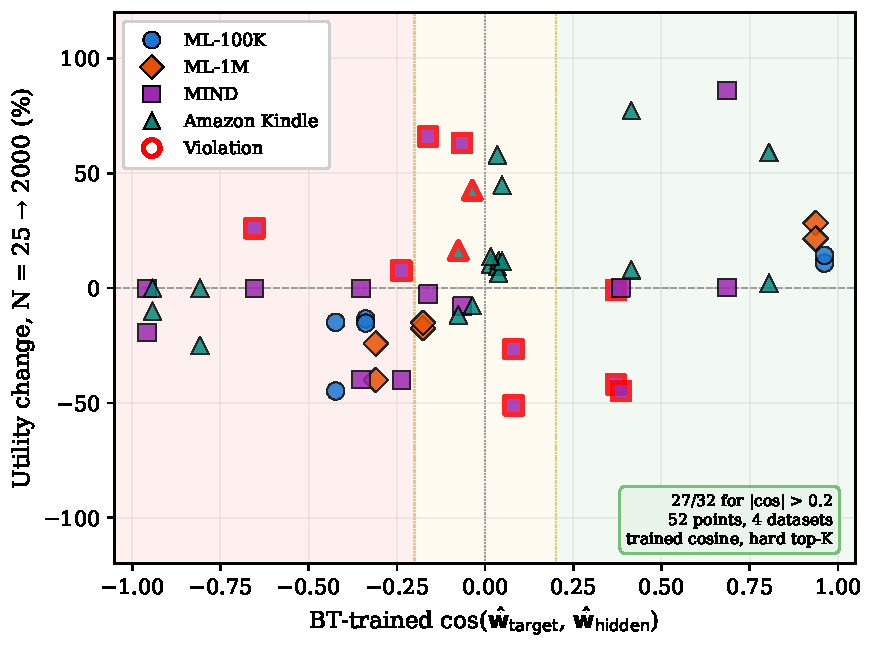
\includegraphics[width=\linewidth]{figures/fig3_direction_scatter.pdf}
  \caption{Direction condition validation across 4 datasets and
    13 stakeholders (BT-trained cosines, top-$K$ utility change).
    Red shading: $\cos < -0.2$ (predicted degradation). Green:
    $\cos > 0.2$ (predicted improvement). Amber: transition zone.
    Red outlines mark violations. Under top-$K$: 29/32 for
    $|\cos| > 0.2$; the 3 violations (all MIND journalist pairs)
    vanish under softmax $T \geq 1$ (32/32).}
  \label{fig:scatter}
\end{figure}

\subsection{Selection Mechanism Matters}
\label{sec:selection_mechanism}

The direction condition is a statement about expected utility under the
learned score distribution (\cref{eq:expected_util}). When content
selection uses a hard top-$K$ cutoff instead of a soft weighting, the
condition can reverse. We test this with a temperature sweep: for each
(target, hidden) pair, we evaluate hidden utility under softmax
selection at temperatures $T \in \{0.001, \ldots, 10\}$ and compare
against hard top-10.

On MIND, hard top-10 matches the direction condition on 11 of~14
strong-cosine pairs (79\%). At $T = 1.0$, the match rate rises to
14/14 (100\%). On both MovieLens datasets and Amazon, both mechanisms
give 100\% at $|\cos| > 0.2$. The transition occurs between
$T = 0.5$ and $T = 1.0$.

The mechanism: hard top-$K$ concentrates on items where the target
stakeholder scores highest. For hidden stakeholders with high utility
variance near the selection boundary, these items can be specifically
the ones where target and hidden \emph{locally} diverge, despite their
\emph{global} cosine being positive. Softmax weighting averages over
this local divergence, recovering the global prediction. This is a form
of extremal Goodhart~\cite{skalse2024goodhart} operating \emph{within}
the positive-cosine regime: the selection mechanism, not the cosine
geometry, drives the reversal.

The practical implication is that the direction condition is directly
applicable to platforms using probability-weighted or temperature-scaled
ranking (as most modern recommender systems do). For systems using hard
top-$K$ selection, stakeholders with high utility variance on
borderline items should be monitored explicitly.

\subsection{The MovieLens Goodhart Curve}

\Cref{fig:goodhart} shows the Goodhart effect in action on MovieLens.
Three stakeholder utility curves are plotted as a function of training
pairs~$N$, normalized to percentage change from the $N = 25$ baseline.
On both ML-100K (\cref{fig:goodhart}a) and ML-1M
(\cref{fig:goodhart}b), user and platform utilities increase
monotonically ($+14\%$ by $N = 2{,}000$), while diversity utility
decreases ($-34\%$ on ML-100K, $-46\%$ on ML-1M). The cosine values
in the legend predict the direction: positive cosine leads to an
upward curve, negative cosine to a downward curve.

\begin{figure*}[t]
  \centering
  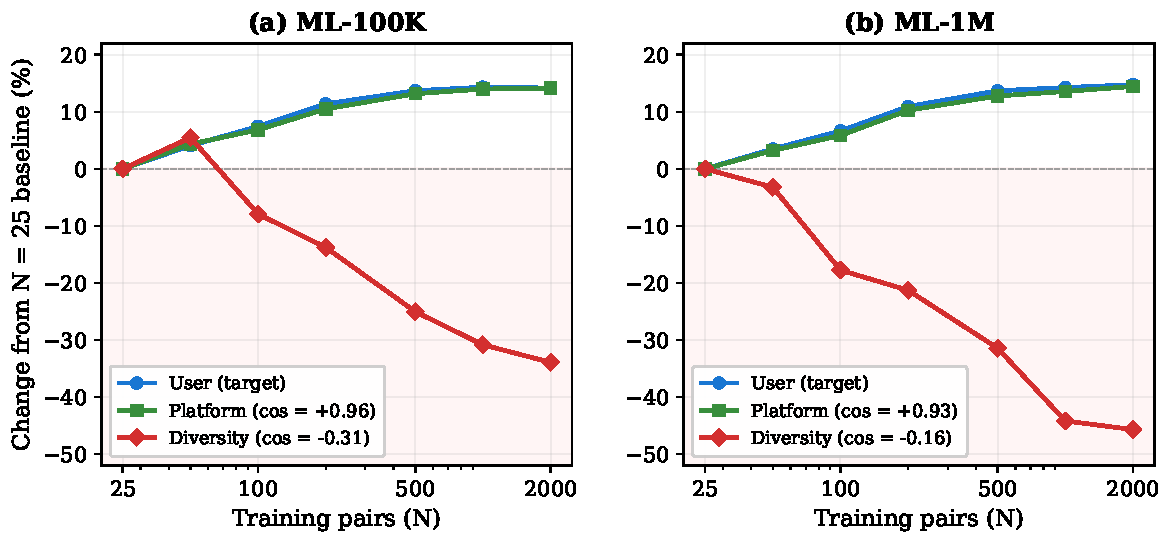
\includegraphics[width=\textwidth]{figures/fig2_goodhart_curves.pdf}
  \caption{Multi-stakeholder Goodhart effect on MovieLens. User and
    platform (cosine $> 0$ with target) improve monotonically.
    Diversity (cosine $< 0$) degrades. Same experiment, same data,
    opposite outcomes predicted by the cosine sign.
    \textbf{(a)}~ML-100K ($D = 19$, 1{,}305 movies).
    \textbf{(b)}~ML-1M ($D = 19$, 3{,}347 movies).}
  \label{fig:goodhart}
\end{figure*}

The mechanism is extremal Goodhart~\cite{skalse2024goodhart}, but
through a different channel than RL policy optimization. BT
preference learning converges to the target utility direction at a
rate determined by~$N$. On a finite content pool, more precise
convergence causes the top-$K$ selection to concentrate on content
that scores high on the target but poorly on anti-correlated
stakeholders. There are no distributional tails to exploit; the
content pool is fixed. The effect is driven entirely by the angle
between stakeholder utility directions.

\subsection{The Synthetic Null Case}

On the synthetic benchmark built on X's 18-action engagement space
(\cref{sec:setup}), all three stakeholder pairs have positive cosine
similarity: user--platform $= +0.89$, user--society $= +0.84$,
platform--society $= +0.51$. The direction condition predicts no
Goodhart for any pair---and under utility-based evaluation, this is
exactly what we observe: society utility \emph{improves} from $3.21$
($N = 25$) to $5.34$ ($N = 2{,}000$), a $+67\%$ increase.

The absence of Goodhart on synthetic data is itself informative: the
synthetic benchmark's stakeholder geometry (all $\cos > 0$)
represents a regime where more data is universally beneficial. The
MovieLens benchmark, where user--diversity $\cos \approx -0.3$,
represents the opposing regime. The direction condition explains both.
A standard frontier distance metric (Hausdorff distance) gives a
different and misleading picture on this data; we address this
discrepancy in \cref{sec:hausdorff}.

%═══════════════════════════════════════════════════════════════════
\section{Why the Condition Holds: Low-Rank Weight Space}
\label{sec:lowrank}
%═══════════════════════════════════════════════════════════════════

The direction condition's predictive power rests on BT-learned weight
vectors being geometrically constrained. We present two lines of
evidence: (1)~the loss function is irrelevant given labels, and
(2)~scalarized weight vectors lie approximately in the span of
per-stakeholder vectors.

\subsection{Labels, Not Loss}

If two loss functions train on identical preference pairs, do they
converge to the same weights? We train Bradley-Terry, margin-BT
($m{=}0.5$), and calibrated-BT ($\lambda{=}1.0$) on each stakeholder
with 5~seeds and measure the \emph{within-loss cosine}: the mean
pairwise cosine similarity of weight vectors trained by different
losses on the same labels.

\begin{table}[t]
  \caption{Within-loss cosine similarity (mean $\pm$ std across 5
    seeds). Values above 0.90 indicate that the loss function has
    negligible effect on the learned direction given identical labels.}
  \label{tab:within_loss}
  \centering\small
  \begin{tabular}{llr}
    \toprule
    \textbf{Dataset} & \textbf{Stakeholder} &
      \textbf{Within-loss cos} \\
    \midrule
    ML-100K & user      & $0.957 \pm 0.005$ \\
            & platform  & $0.987 \pm 0.003$ \\
            & diversity & $0.958 \pm 0.006$ \\
    \midrule
    MIND    & reader      & $0.911 \pm 0.007$ \\
            & publisher   & $0.944 \pm 0.006$ \\
            & advertiser  & $0.965 \pm 0.006$ \\
            & journalist  & $0.847 \pm 0.007$ \\
            & civic\_div. & $0.824 \pm 0.019$ \\
    \midrule
    Amazon  & reader          & $0.940 \pm 0.005$ \\
            & publisher       & $0.961 \pm 0.006$ \\
            & indie\_author   & $0.890 \pm 0.016$ \\
            & premium\_seller & $0.975 \pm 0.003$ \\
            & diversity       & $0.909 \pm 0.008$ \\
    \bottomrule
  \end{tabular}
\end{table}

\Cref{tab:within_loss} shows the results. On MovieLens ($D{=}19$),
all three stakeholders exceed 0.95: the loss function is
essentially irrelevant. On MIND and Amazon ($D \geq 32$), 11 of~13
stakeholders exceed 0.89. The two exceptions---MIND journalist
(0.847) and civic\_diversity (0.824)---have the sparsest weight
vectors in the dataset (12 and~17 nonzero dimensions out of~35
respectively). The core claim holds: \emph{stakeholder
differentiation comes from the training labels, not the loss
function}, with the qualification that very sparse stakeholders on
high-dimensional features show weaker convergence.

\subsection{Low-Rank Composition}

If BT-learned weight vectors are constrained to a low-dimensional
subspace, then the cosine geometry that drives the direction condition
is itself low-dimensional. We test this by training scalarized models
(BT on mixed-stakeholder preferences) and projecting each learned
weight vector onto the span of the per-stakeholder weight vectors.

\begin{table}[t]
  \caption{Composition analysis: scalarized weight vectors projected
    onto the per-stakeholder span. Higher projection cosine indicates
    tighter low-rank structure.}
  \label{tab:composition}
  \centering\small
  \begin{tabular}{lrrrr}
    \toprule
    \textbf{Dataset} & $\boldsymbol{K}$ & $\boldsymbol{D}$ &
      \textbf{Mean proj.\ cos} & \textbf{Frac.\ $> 0.95$} \\
    \midrule
    ML-100K       & 3 & 19 & 0.979 & 21/21 \\
    MIND-small    & 5 & 35 & 0.893 & 30/121 \\
    Amazon Kindle & 5 & 32 & 0.877 & 31/121 \\
    \bottomrule
  \end{tabular}
\end{table}

The low-rank structure is present on all datasets but varies in
tightness (\cref{tab:composition}). On MovieLens, nearly all
scalarized models project onto the 3-stakeholder span with cosine
above~0.95. On MIND and Amazon, the mean projection cosine drops to
${\sim}0.88$---still far above the random baseline for a
$K$-dimensional subspace in $D$-dimensional space (${\sim}0.6$), but
no longer tight enough to claim that scalarization is fully contained
in the per-stakeholder span. The weaker structure on high-$K$,
high-$D$ datasets is consistent with the additional degrees of freedom
available to scalarized training: with 5~stakeholders and 32--35
features, the mixing-weight simplex is large enough for the optimizer
to find directions outside the per-stakeholder span.

The practical implication: the direction condition's success is not
contingent on an exact low-rank decomposition. Even on datasets where
the projection cosine is~0.88, the trained cosine between stakeholders
is sufficient to predict hidden utility direction (32/32 under softmax,
\cref{sec:direction}). The low-rank structure \emph{explains} why the
condition works---BT training is geometrically constrained---but the
condition holds more broadly than the low-rank claim alone would
predict.

%═══════════════════════════════════════════════════════════════════
\section{Practical Implications}
\label{sec:practical}
%═══════════════════════════════════════════════════════════════════

\subsection{Data Budget for Hidden Stakeholder Recovery}

If the direction condition identifies \emph{which} hidden
stakeholders are harmed, a natural follow-up is: how much data
from the hidden stakeholder is needed to mitigate the harm?

We run leave-one-stakeholder-out (LOSO) experiments across three
real datasets (ML-100K, MIND, Amazon Kindle), hiding each
stakeholder in turn. At $N = 0$ hidden-stakeholder preference pairs,
the LOSO regret (utility gap from the full-information Pareto
frontier) is the baseline harm. We then add
$N \in \{25, 50, 100, 200, 500\}$ hidden-stakeholder pairs and
retrain, measuring the \emph{recovery}: the fraction of baseline
regret eliminated. We report the preference budget $N_{50\%}$ and
$N_{80\%}$ --- the minimum $N$ needed to reach 50\% and 80\%
recovery, interpolated across the sweep.

Across 13 (dataset, hidden stakeholder) configurations, the
\textbf{median $N_{50\%}$ is 33~pairs} and the \textbf{median
$N_{80\%}$ is 104~pairs}. The practical cost is modest: 33
preference pairs can be collected from 7 annotators making 5
pairwise comparisons each. For most hidden stakeholders, a
modest investment detects and substantially mitigates hidden harm.

The variance is large. On Amazon Kindle, hiding reader requires
only 14~pairs for 50\% recovery, while hiding publisher requires
368---reflecting publisher's strong anti-alignment with every other
stakeholder ($\cos < -0.5$ with 2 of~4 others). One configuration
(ML-100K, hide user) does not reach 50\% within the 500-pair sweep,
because the remaining stakeholders (platform, diversity) already
proxy for user well ($\cos(\text{user}, \text{platform}) = +0.95$).
The full per-stakeholder breakdown is in \cref{app:data_budget}.

% TODO: Regenerate fig5 with N-for-target framing across datasets
\begin{figure}[t]
  \centering
  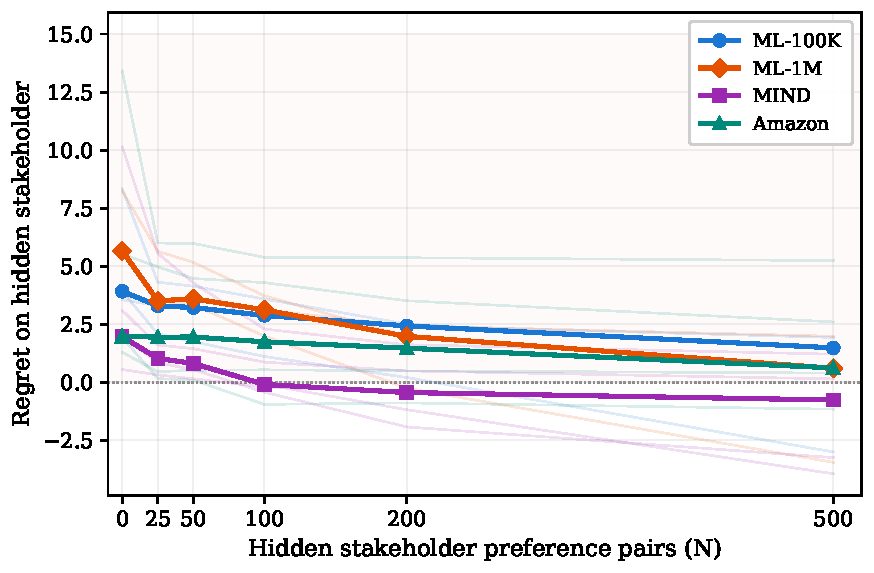
\includegraphics[width=\linewidth]{figures/fig5_data_budget.pdf}
  \caption{Data budget for hidden stakeholder recovery across
    13~configurations on 3~datasets. Median budget: 33~pairs for
    50\% recovery, 104~pairs for 80\%. Worst case: $> 500$ pairs
    for stakeholders with strong substitutes in the observed set.}
  \label{fig:budget}
\end{figure}

\subsection{Audit Toolkit Applied to X}
\label{sec:audit}

The direction condition reduces multi-stakeholder Goodhart risk to
a single observable: the sign of
$\cos(\mathbf{w}_{\text{platform}}, \mathbf{w}_{\text{society}})$.
For X's 18-action space (\cref{tab:actions}), this cosine is
determined almost entirely by how the platform weights negative
actions (blocks, mutes, reports).

\Cref{fig:audit} shows the relationship. When the platform treats
negative actions as positive engagement (weight $> 0$), the
cosine with society drops below zero and the direction condition
predicts Goodhart. When negative actions carry any penalty (weight
$< 0$), the cosine remains positive and no Goodhart is predicted.

We evaluate five platform configurations on the synthetic
benchmark (\cref{tab:scenarios}):

\begin{table}[t]
  \caption{Audit scenarios on X's 18-action space. The single
    variable determining Goodhart risk is how the platform weights
    negative actions. $\alpha$: negativity aversion
    (\cref{eq:synth_utility}).}
  \label{tab:scenarios}
  \centering\small
  \begin{tabular}{lrrll}
    \toprule
    \textbf{Scenario} & $\boldsymbol{\alpha}$ &
      \textbf{cos(plat, soc)} & \textbf{Risk} \\
    \midrule
    Pure engagement     & 0 & $-0.31$ & Goodhart \\
    2023 Phoenix        & 0.3 & $+0.51$ & Low \\
    User-aligned        & 1.0 & $+0.84$ & Low \\
    Safety-first        & 2.0 & $+0.97$ & Low \\
    \bottomrule
  \end{tabular}
\end{table}

The 2023 open-sourced Phoenix code~\cite{xalgorithm2023} had
explicit negative weights (e.g., block\_author $= -1.5$, report
$= -3.0$), placing it safely above the threshold. The 2026
Grok-based system~\cite{xalgorithm2026} replaced explicit weights
with learned embeddings, making the same audit impossible without
additional disclosure: the cosine between the system's implicit
optimization target and a societal utility direction cannot be
computed from the released code alone.

\begin{figure}[t]
  \centering
  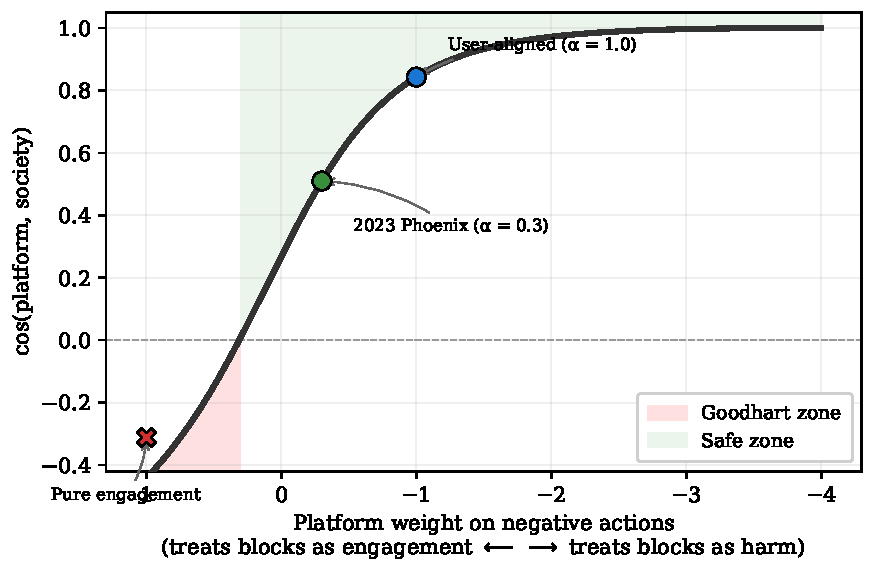
\includegraphics[width=\linewidth]{figures/fig4_audit_threshold.pdf}
  \caption{Audit threshold for X's 18-action space. The curve
    shows $\cos(\text{platform}, \text{society})$ as a function of
    the platform's weight on negative actions. Goodhart zone (red):
    negative actions treated as positive engagement. Safe zone
    (green): any negative penalty suffices. Markers show specific
    platform configurations.}
  \label{fig:audit}
\end{figure}

\paragraph{A five-step audit procedure.}

For regulators operating under the EU Digital Services Act or
similar transparency frameworks, we propose:
\begin{enumerate}
  \item \textbf{Extract} the platform's optimization objective as a
    weight vector over observable user actions.
  \item \textbf{Define} a societal utility direction
    $\mathbf{w}_{\text{soc}}$ (e.g., negative weight on
    block/report signals).
  \item \textbf{Compute}
    $\cos(\mathbf{w}_{\text{platform}},
    \mathbf{w}_{\text{society}})$.
  \item \textbf{If} $\cos < 0$: the direction condition predicts
    that more training data \emph{increases} societal harm.
    Escalate.
  \item \textbf{If} $\cos > 0$: no directional Goodhart is
    predicted. Periodic monitoring suffices.
\end{enumerate}

Step~1 is the bottleneck. For systems with explicit weights (2023
Phoenix), the audit is immediate. For systems with learned
representations (2026 Grok), Step~1 requires the platform to
disclose either the effective weight vector or sufficient
information to compute the cosine. The direction condition provides
a concrete, falsifiable quantity that regulators can demand.

\subsection{Selection Mechanism Independence}

The diversity parameter~$\delta$ (\cref{sec:eval}) provides a
structural safeguard independent of stakeholder utility
specification. Because $\delta$ controls the tradeoff between
score-based and diversity-based content selection at the mechanism
level, it is orthogonal to the stakeholder weight vectors: changing
$\delta$ does not change the cosine between any pair of
stakeholders.

In our experiments, the rank ordering of operating points on the
Pareto frontier is perfectly stable under utility weight
perturbation (rank stability $= 1.0$ across all conditions). This
means that even if individual stakeholder weights are misspecified,
the diversity knob still provides a reliable control dimension. The
design principle: recommendation systems should maintain at least
one structural control parameter that is independent of the
learned objective.

%═══════════════════════════════════════════════════════════════════
\section{Methodological Note: Hausdorff Distance and False Positive Goodhart}
\label{sec:hausdorff}
%═══════════════════════════════════════════════════════════════════

% TODO: Metric correction
\textit{[Hausdorff correction placeholder.]}

%═══════════════════════════════════════════════════════════════════
\section{Limitations}
\label{sec:limitations}
%═══════════════════════════════════════════════════════════════════

% TODO: Scale gap, magnitude, linear utilities, transition zone
\textit{[Limitations placeholder.]}

%═══════════════════════════════════════════════════════════════════
\section{Conclusion}
\label{sec:conclusion}
%═══════════════════════════════════════════════════════════════════

% TODO: Direction condition, toolkit, honest limits
\textit{[Conclusion placeholder.]}

%═══════════════════════════════════════════════════════════════════
\bibliographystyle{plain}
\bibliography{references}
%═══════════════════════════════════════════════════════════════════

\appendix

% TODO: Fill appendix sections
\textit{[Appendix placeholder.]}

\end{document}
